\section{Diskretisierung und Implementierung}
\subsection{Basics}
\begin{figure}[h!]
	\begin{minipage}{0.5\linewidth}
		\centering
		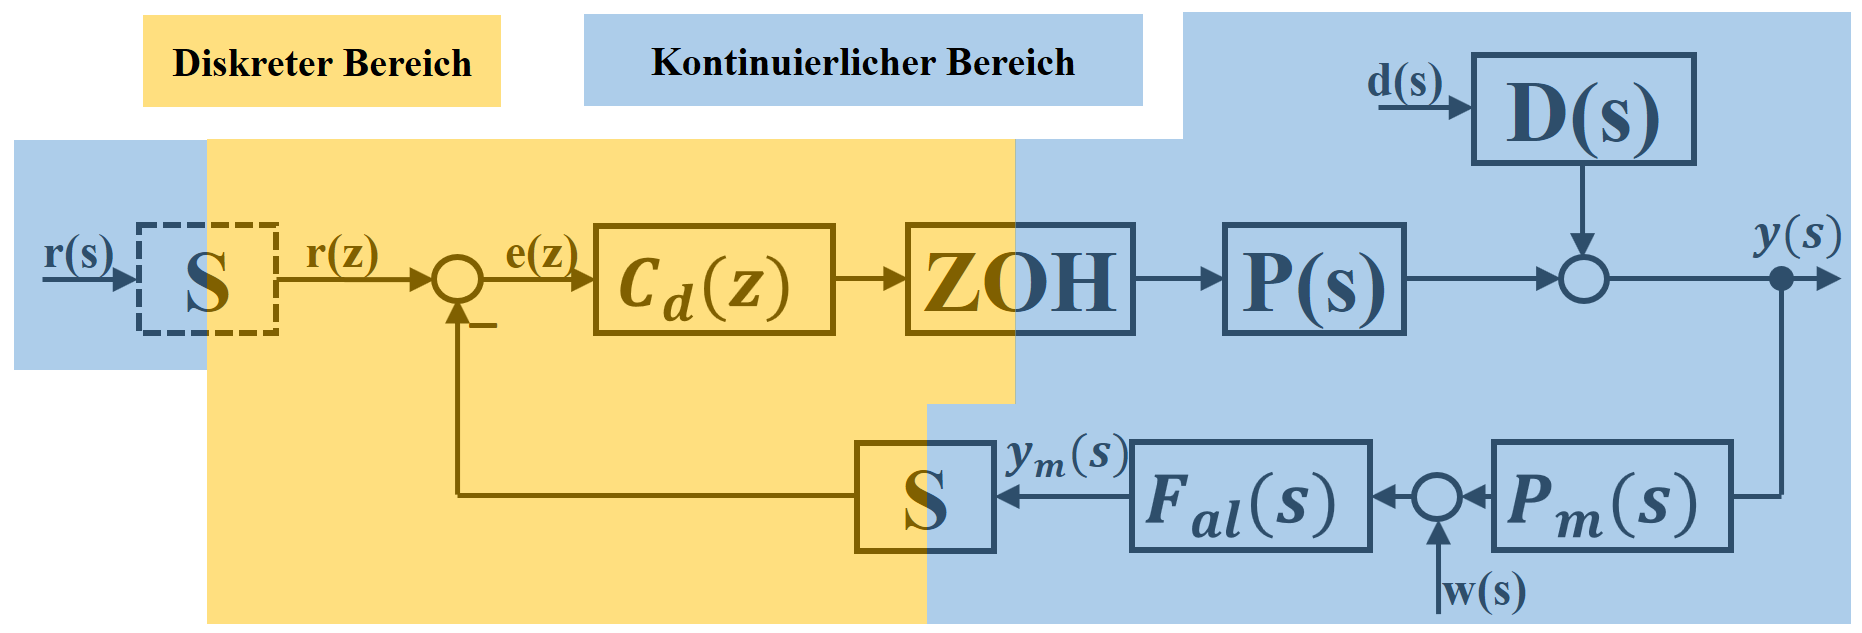
\includegraphics[width=.9\linewidth]{bilder/DiskretesSystem}
		\label{fig:diskretessystem}
	\end{minipage}
	\begin{minipage}{0.45\linewidth}
		\footnotesize
		\begin{tabular}{rl}
			S 						&= Samplingmodul (ADC)\\
			ZOH 					&= Zero Order Hold (DAC)\\
			P(s)					&= Regelstrecke\\
			$\text{C}_d$			&= diskreter Regler\\
			$\text{F}_{al}$			&= anti aliasing Filter\\
			$\text{P}_m$			&= Sensorübertragungsfunktion\\
			w						&= Noise Signal zum Sensor\\
			$\text{P}_m+\text{w}$	&= Sensor Modell\\
			d						&= Noise von der Regelstrecke\\
			D						&= Shaping Filter
		\end{tabular}
	\end{minipage}
\end{figure}
\begin{itemize}
	\item Hier ist nicht mehr linke Halbebene ausschlaggebend über stabilität, sondern ob alle Pol- und Nullstellen innerhalb des Einheitskreises liegen
\end{itemize}

\subsection{Diskretisierung von Reglern}
\begin{itemize}
	\item In Zeitdomain $\dot{y}(t) $ wird in Laplace-Raum zu $sy(s)$ in diskretisierten Raum entspricht dies $\dot{y(t)}\sim\frac{y(kt)-y(kt+T)}{T}$
	\item Die Bildung der Differenzengleichung erfolgt mit $C(z) = \frac{y(z)}{e(z)}$
\end{itemize}
\subsubsection{Diskretisierungsmethoden}
\begin{itemize}
	\item Entsprechend in der Übertragungsfunktion alle $s$ mit dem entsprechenden Term der Transformation ersetzten. Dabei ist $T$ die Abtastzeit
	\item Die Bilineare Transformation bildet die linke halbebene in den Einheitskreis ab. (siehe Abbildung \ref{fig:Tustin})
	\begin{itemize}
		\item Somit ist garantiert, dass stabile Regler auch im diskreten stabil bleiben.
	\end{itemize}
	\item Pole-Zero-Matching: Wenn der Regler unendlich Nullstellen hat, können diskrete Pole bei -1 angenommen werden
\end{itemize}
\begin{align*}
	\text{\textbf{Vorwärtseuler}} \qquad & s=\frac{z-1}{T}\\
	\text{\textbf{Rückwärtseuler}} \qquad & s=\frac{z-1}{Tz}\\
	\text{\textbf{Tustin / Bilinear}} \qquad & s=\frac{2}{T}\frac{z-1}{z+1}\\
	\text{\textbf{Zero-Order-Hold}} \qquad& G(z) = \frac{z-1}{z}\mathcal{Z}\left\{\mathcal{L}^{-1}\left\{\frac{G(s)}{s}\right\}\right\}\\
	\text{\textbf{Pole and zero Matching}} \qquad & z=e^{s\cdot T}
\end{align*}
\begin{figure}[h!]
	\centering
	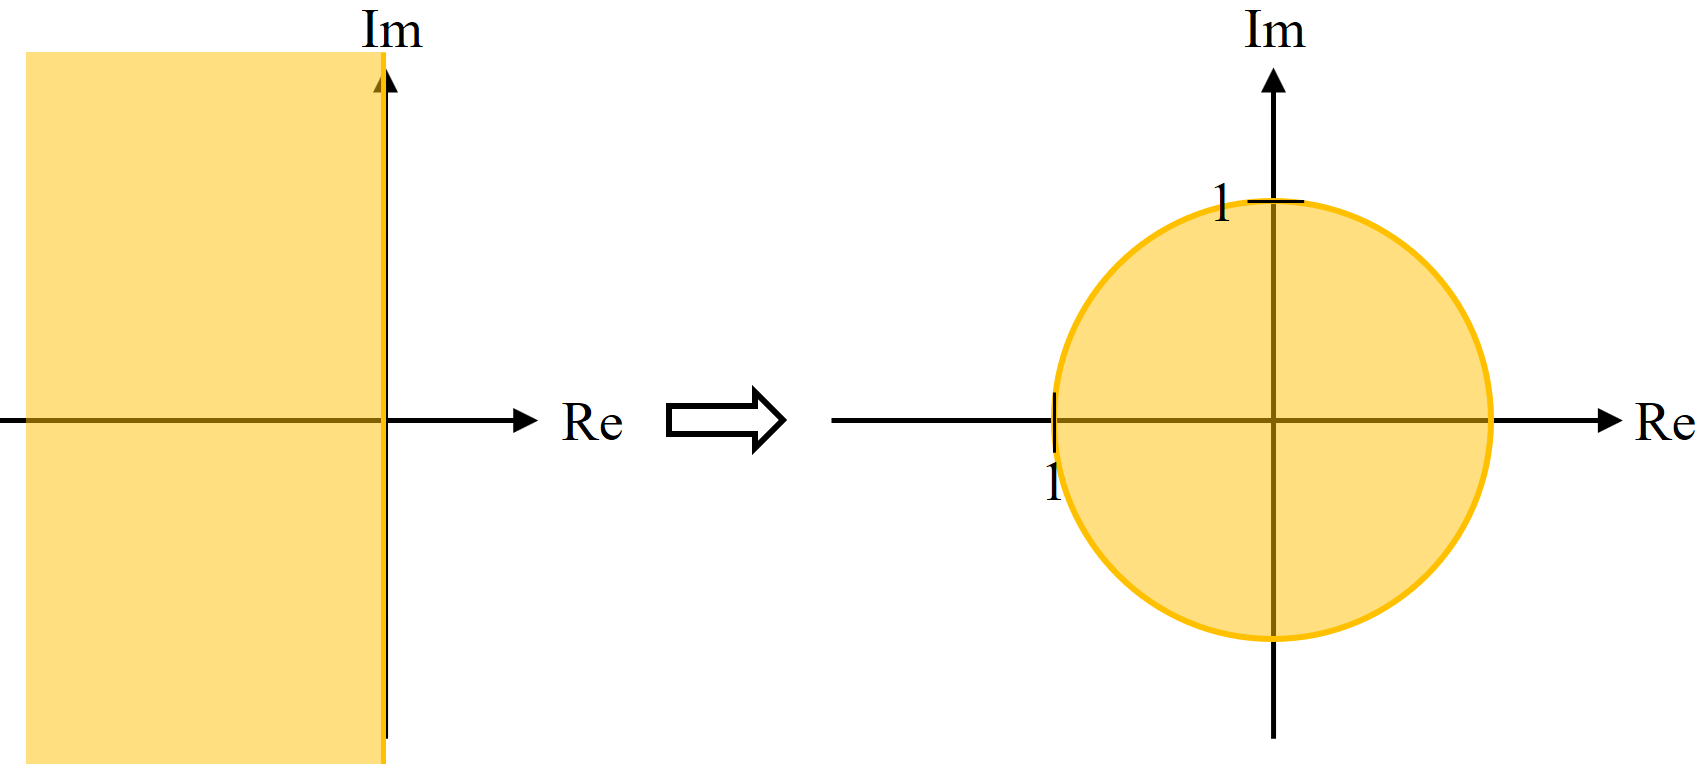
\includegraphics[width=0.3\linewidth]{bilder/Tustin}
	\caption{Tustin-Verfahren führt linke Halbebene in Einheitskreis über}
	\label{fig:Tustin}
\end{figure}

\subsubsection{Wahl der Sampling Time}
\begin{itemize}
	\item Gründe für Maximierung der sampling Time
	\begin{itemize}
		\item Pole entfernen sich von 1, somit wird controllaw nummerisch stabiler. (weniger anfällig für Quantisierungsfehler)
		\item Hardware muss weniger leistungsfähig sein $\Rightarrow$ günstiger
		\item Differenzierende Regler funktionieren besser (Glättung des Signals, da Ableitung über längere Zeitperiode)
	\end{itemize}
	\item Gründe für Minimierung der sampling Time
	\begin{itemize}
		\item Wenn A/D und D/A wandler synchronisiert sind, führt dies zu einer kleineren Totzeit
		\item Bei Verwendung eines Anti-Aliasing-Filters (für verrauschte Signale) ist der Phasenverlust kleiner
		\item Je kleiner die Sampling Time, desto weniger Phasenverlust durch das ZOH-Glied
	\end{itemize}
	\item Maximale Frequenz: Signal darf keine Frequenzen enthalten die grösser sind als halbe Abtastfrequenz
	\begin{itemize}
		\item [] $f_\text{max}\leq \frac{1}{2}\cdot f_\text{Abtast}$
		\item Kann hergeleitet werden mit Shannon-Nyquist
	\end{itemize}
	\item Das Shannon-Sampling Theorem besagt: Sampling Frequenz (in rad) soll grösser sein als $20\omega_d$ des offenen Regelkreises ($\omega_d$ = Durchtrittsfrequenz)
\end{itemize}

\subsection{Windup und weitere Gefahren}
\begin{itemize}
	\item Regler summiert Fehler zu schnell auf (da Regelstrecke langsam und Abtastzeit hoch ist)
	\item Wenn zwei Pole bei einem digitalen Regler zu nahe zusammen liegen, muss mit Quantisierungsproblemen gerechnet werden. 
\end{itemize}
\newpage